\section{申请流程(此部分仅供流程介绍,不在最终提交材料中)}

\subsection{注册申请账号}

点击下面的链接即可进入版权保护中心的用户中心登录页面：

\url{https://register.ccopyright.com.cn/account.html?current=soft_register}

注册完成后需要进行实名认证，需要大约3个工作日审核。审核完成后，即可开始登记软件著作权。


\subsection{软著登记}


\begin{figure}[H]
	\centering
	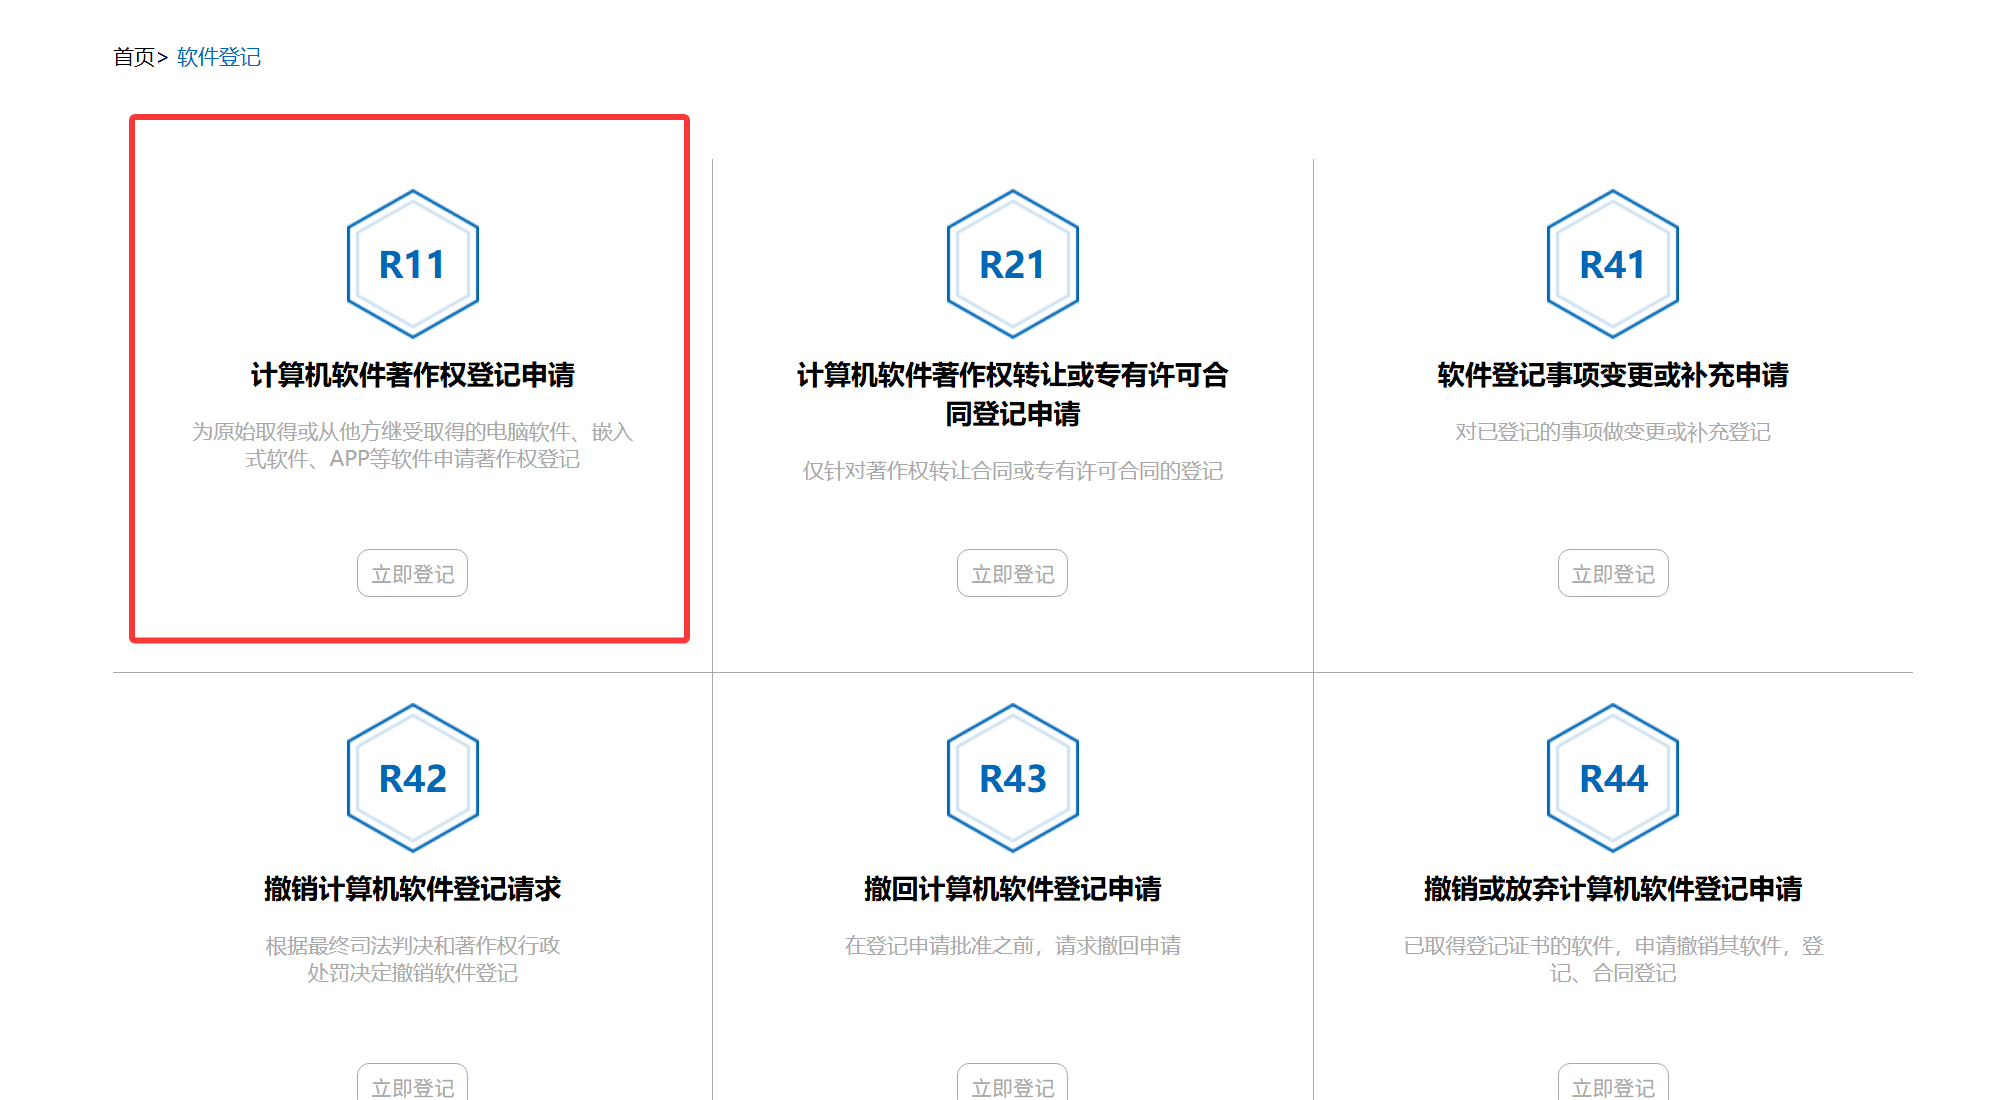
\includegraphics[width=0.99\linewidth]{figures/screenshot001}
	\caption{软件登记页面}
	\label{fig:screenshot001}
\end{figure}

登记类型选择R11，登记证书类型为原始取得。


\newpage
\section{软件简介}

\textbf{下述内容均为材料中必须有的内容，可以在这个基础上增加，但是不能减少必要内容。}

\subsection{编写目的}

\subsection{使用对象}

\subsection{使用范围}


\newpage
\section{产品概述}

\subsection{产品框架}

\subsection{系统架构}

\subsection{模块描述}

\newpage
\section{软件开发说明}

\subsection{软件界面}

\subsection{交互说明}

\subsection{对外接口说明}

\subsection{数据说明}

\subsection{函数实现说明}

\subsection{用户操作接口说明}

\newpage
\section{软件测试说明}

\subsection{手动测试说明}

\subsection{边界测试说明}

\newpage
\section{软件总结与未来设计目标}

\subsection{软件总结}





\subsection{未来设计目标}






